% BREDEX LaTeX Template
%  \documentclass is either ``bxreport'' or ``bxarticle''
%% %                 option is bxpaper
%% \documentclass{bxarticle}
%% % ----------------------------------------------------------------------
%% \begin{document}
%% \title{}
%% \author{}
%% % \author*{Hauptautor}{Liste der Nebenautoren}
%% \maketitle
%% % ----------------------------------------------------------------------
%% \bxversion{0.1}
%% %\bxdocinfo{STATUS}{freigegeben durch}{freigegeben am}{Verteilerliste}
%% \bxdocinfo{DRAFT}{}{}{}
%% % ----------------------------------------------------------------------

%% \end{document}
\begin{enumerate}
\item Create a \gdproject{} in the same way as described at the beginning of this chapter \bxpref{tutorialsetup}, but with a different \gdproject{} name. 
\item Select:\\
\bxmenu{Project}{Import}{}\\
and browse to the \gdproject{} \bxname{unbound\_modules\_concrete}.  It is located under \bxname{aut/testCaseTemplate} in the \app{} installation. 
\item Do not select the option to open the \gdproject{} immediately after import, but do make sure you import the whole \gdproject{}, and not just its \gdcases{}.
\item Open the \gdproject{} properties dialog:\\
\bxmenu{Project}{Properties}{}
\item Select \bxname{Used Projects} from the left-hand side (\bxfigref{TutUsedProjects}). Select the highest available version of the \bxname{unbound\_modules\_concrete} \gdproject{} and add it to the list of reused \gdprojects{}.

 \begin{figure}[h]
\begin{center}
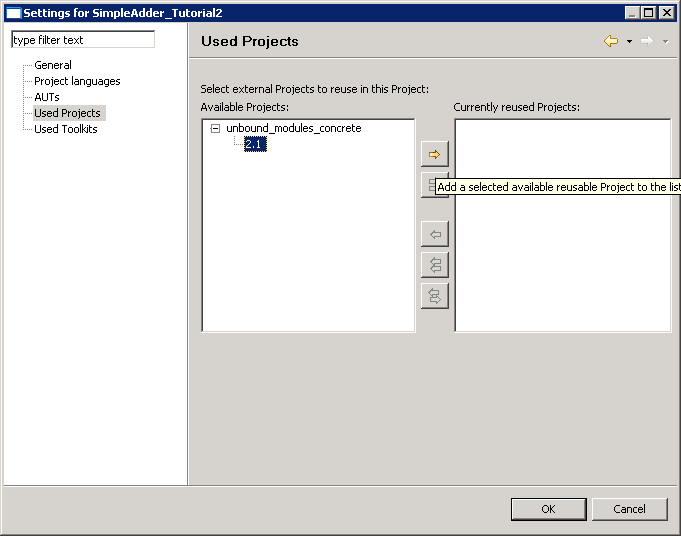
\includegraphics[width=12cm]{Tutorials/PS/TutUsedProjects}
\caption{The used project dialog}
\label{TutUsedProjects}
\end{center}
\end{figure}

\item Click \bxcaption{OK}. 

In the \gdtestcasebrowser{}, you will see the reused \gdproject{} you just selected. It is grayed out, because it is a reference to the original \gdproject{}. In essence, it is a library of highly reusable \gdcases{} which you can use in other tests. 


\end{enumerate}
